\documentclass[12pt,journal,compsoc,onecolumn]{IEEEtran}
\usepackage{graphicx}
\usepackage{cite}
\usepackage{url}
\usepackage{caption}

\providecommand{\PSforPDF}[1]{#1}
\newcommand{\um} {$\mu$m}
\newcommand{\uW} {$\mu$W}

\newcommand\MYhyperrefoptions{bookmarks=true,bookmarksnumbered=true,
pdfpagemode={UseOutlines},plainpages=false,pdfpagelabels=true,
colorlinks=true,linkcolor={black},citecolor={black},pagecolor={black},
urlcolor={black},
pdftitle={Third interim report},%<!CHANGE!
pdfsubject={Typesetting},%<!CHANGE!
pdfauthor={Carsten Bruns \& Jakob Toft},%<!CHANGE!
pdfkeywords={High-speed communication, Voltage-mode driver, Low-power 10GB/s}}%<^!CHANGE!

% correct bad hyphenation here
\hyphenation{op-tical net-works semi-conduc-tor}

\usepackage[]{units}
\usepackage{graphicx}
\usepackage{subfigure}

\usepackage{epstopdf}

\usepackage{pgfplots} 
\usepgfplotslibrary{external}
%\tikzexternalize

\usepackage{float}

\begin{document}
%
% paper title
% can use linebreaks \\ within to get better formatting as desired
\title{Design, Analysis and Simulation of an I/O Link\\Final report}

\author{Carsten Bruns
        \& Jakob Toft% <-this % stops a space

%\IEEEcompsoctitleabstractindextext{%
%\begin{abstract}
%\boldmath
%The abstract goes here.
%\end{abstract}


% Note that keywords are not normally used for peerreview papers.
\begin{IEEEkeywords}
High-Speed Data Links, Low-Power 10Gb/s link.
\end{IEEEkeywords}}


% make the title area
\maketitle

\IEEEdisplaynotcompsoctitleabstractindextext
\IEEEpeerreviewmaketitle

\tableofcontents
\listoffigures
\listoftables

\cleardoublepage
\section{Introduction}
\subsection{Choice of project}

\IEEEPARstart{F}{or} this project we have chosen to design, analyse and simulate a Low-power supply-scalable I/O Link operating at 2-10Gb/s.

\cleardoublepage
\section{Design choices and initial investigation of channel}

\subsection{Choice of equalization techniques and resolution} 
\label{ch:equalization_choice}

To evaluate the required equalization for the data link with the given channel, different options were simulated and the resulting eye-diagrams were created. \\
Figure \ref{fig:eyes_10gbs} shows the eye diagram at the RX input for different equalization configurations with the link running at \unit[10]{Gb/s} and \unit[$\pm$1]{V} TX signal swing. For \unit[2]{Gb/s} the resulting eye diagrams are presented in figure \ref{fig:eyes_2gbs}. All eyes are for a sequence of 1000 pseudo-random bits generated by a 7-bit PRBS generator.\\
Without any equalization the eye is closed for the fast case. By adding a single post cursor (2-tap TXPE) the eye gets much more relaxed. The vertical eye opening is approximately \unit[360]{mV} and the horizontal eye opening \unit[68]{ps}. Comparing this with already implemented links, e.g. the PCIe specification which allows a minimum width of \unit[0.4]{UI} and height of \unit[120]{mV} at the reciever \cite{pcie_spec} for the same BER as in this project (10$^{-12}$), it should be feasible to meet the requirements with only this equalization. As the amount of deterministic jitter for the channel is already included in the simulation, a remaining total jitter of \unit[68]{ps} can be introduced by the transmitter and receiver circuits. The required BER results in a Q of 7 and therefore maximal deterministic jitter in Rx and Tx can be approximated as $DJ\leq\unit[68]{ps}-14*RJ$. So for example we could deal with up to \unit[26]{ps} additional DJ for \unit[3]{ps} of random jitter introduced by the circuits.\\
Adding a second post cursor increases the eye opening in both directions a bit. However, this increase is relatively small for the effort required. As we want to implement a low-power link, the additional amount of power consumption required does not justify adding another tap. Using a pre instead of a post cursor leads to worse performance and is therfore not considered any further. For \unit[2]{Gb/s} with reduced signal swing the received eye is already very good even without any equalization, adding one post cursor reduces the ISI even further.\\
Adding other equalization techniques at the receiver could improve the eye opening and therefore the BER further but would also require more power, especially for DFE. As the received signal seems to be good enough with only equalization at the transmitter, we decided to use only TXPE with 2-taps (cursor and one post cursor) as equalization in the system.


%TODO other equalization techniques
%TODO other references?

\begin{figure}[H]
  \centering
  \subfigure[no equalization]
  {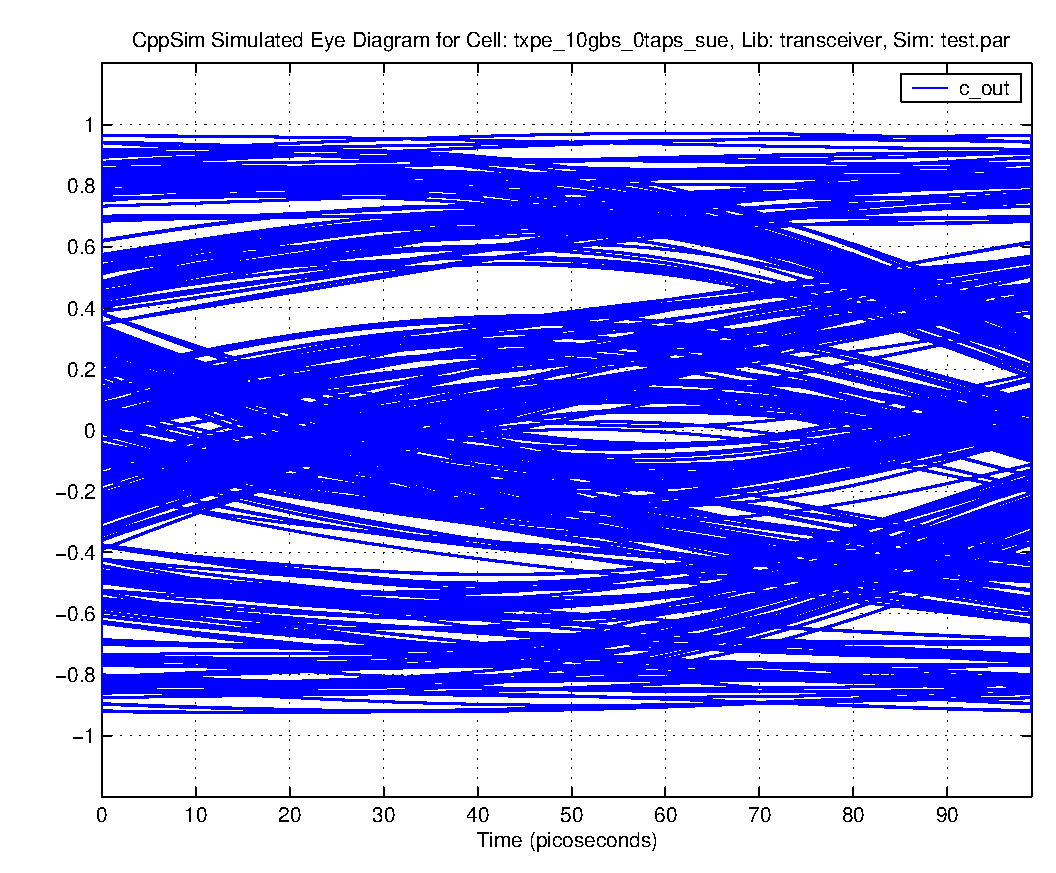
\includegraphics[scale=0.5]{eyes/eye_10gbs_0taps.eps}}
  \subfigure[TXPE, one post cursor]
  {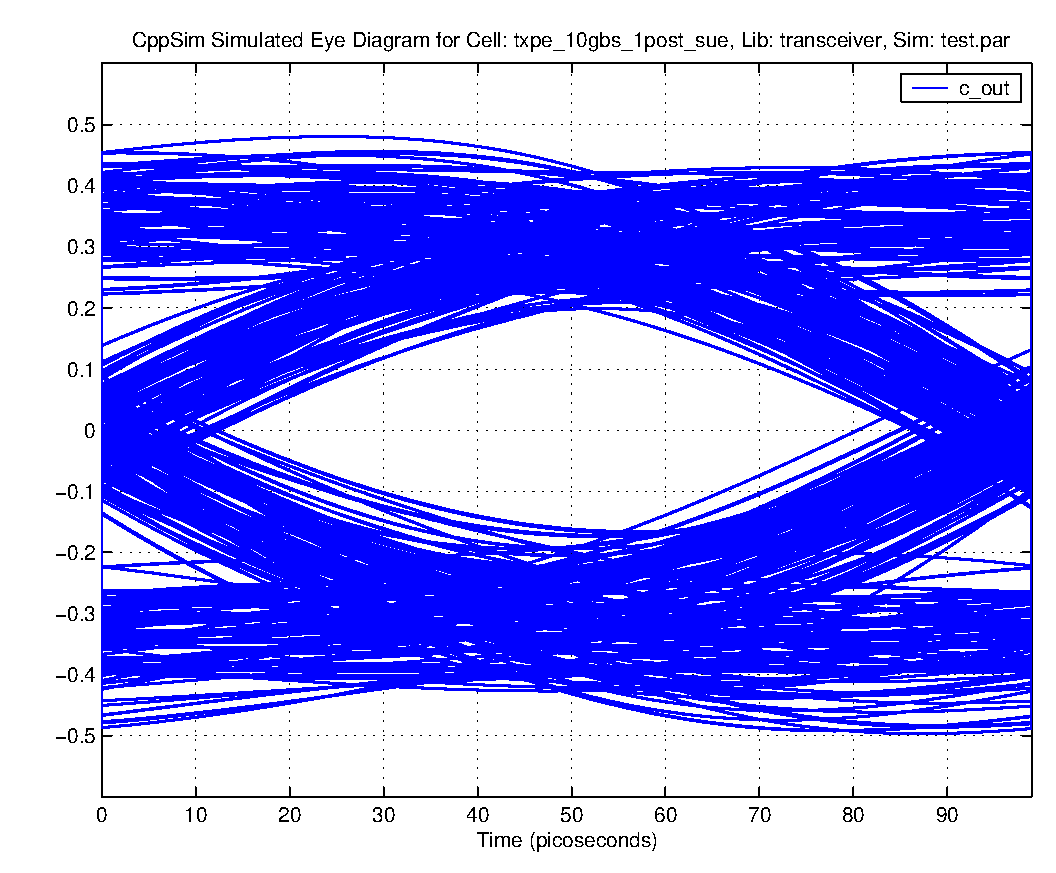
\includegraphics[scale=0.5]{eyes/eye_10gbs_1post.eps}}
  \subfigure[TXPE, two post cursors]
  {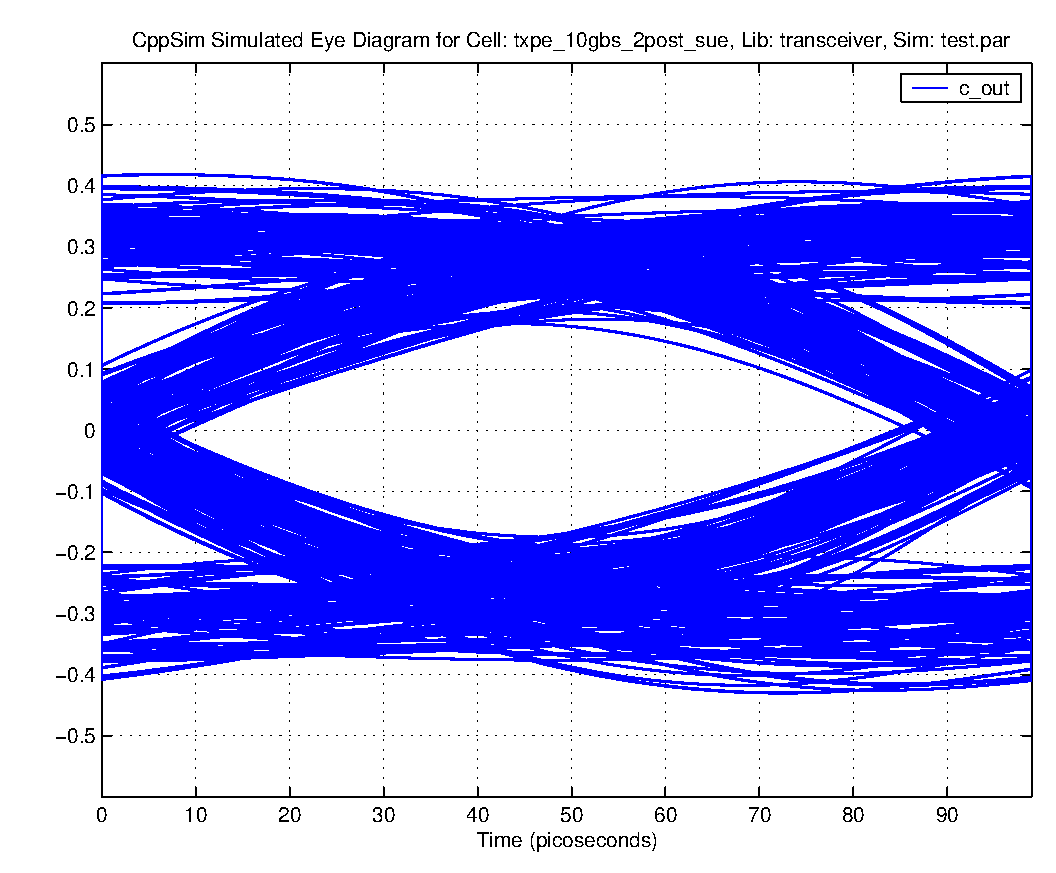
\includegraphics[scale=0.5]{eyes/eye_10gbs_2post.eps}}
  \subfigure[TXPE, one post and one pre cursor]
  {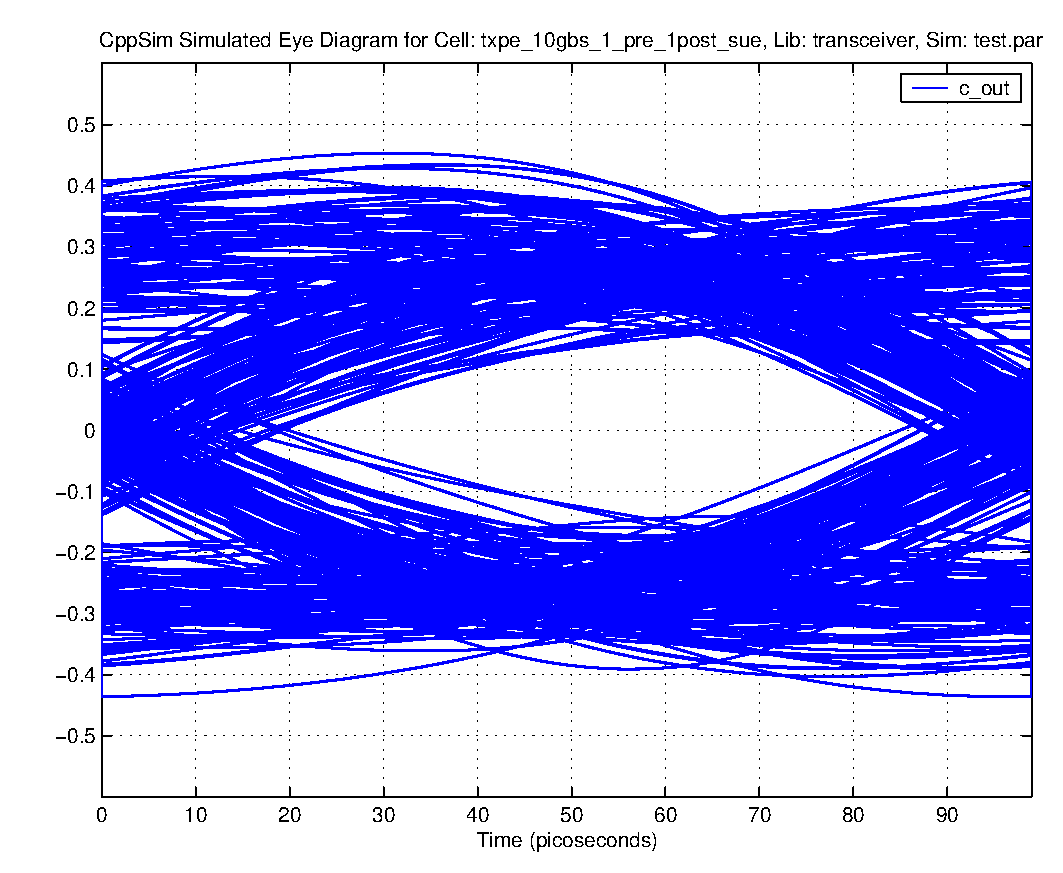
\includegraphics[scale=0.5]{eyes/eye_10gbs_1pre_1post.eps}}
  \caption{Eye diagrams for \unit[10]{Gb/s} and \unit[$\pm$1]{V} TX signal swing}
  \label{fig:eyes_10gbs}
\end{figure}

\begin{figure}[H]
  \centering
  \subfigure[no equalization]
  {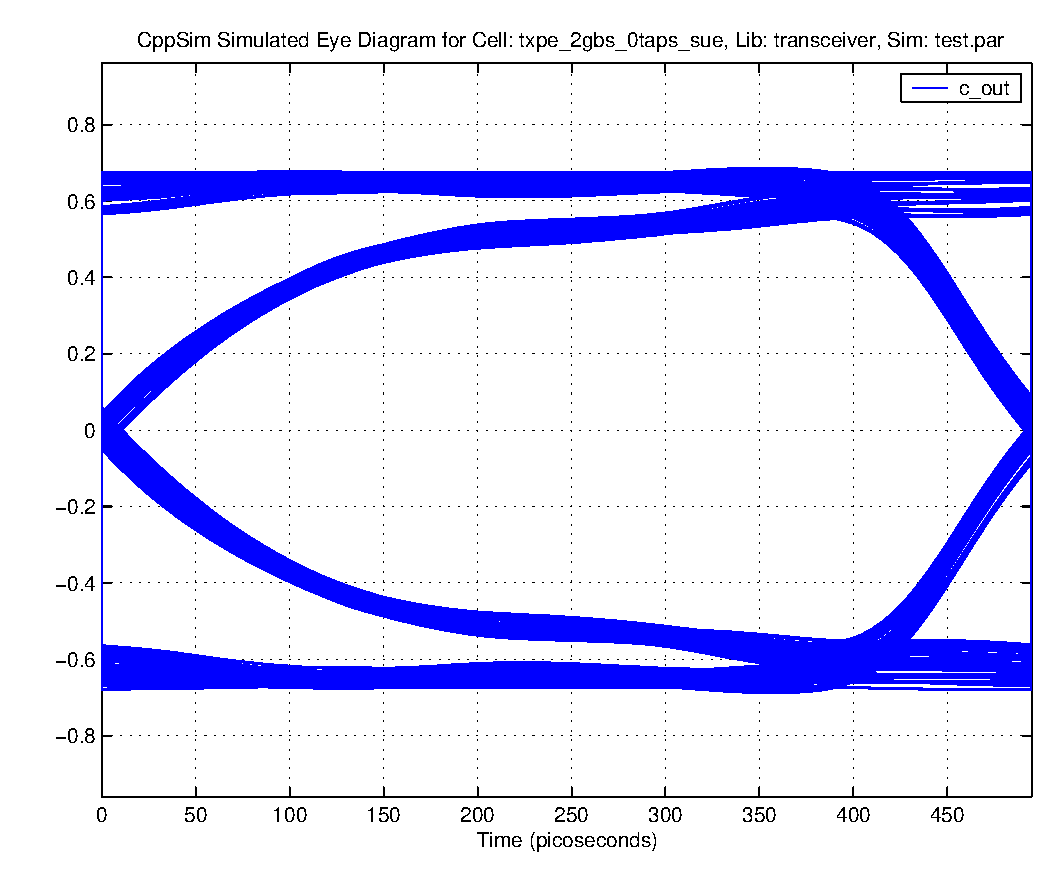
\includegraphics[scale=0.5]{eyes/eye_2gbs_0taps.eps}}
  \subfigure[TXPE, one post cursor]
  {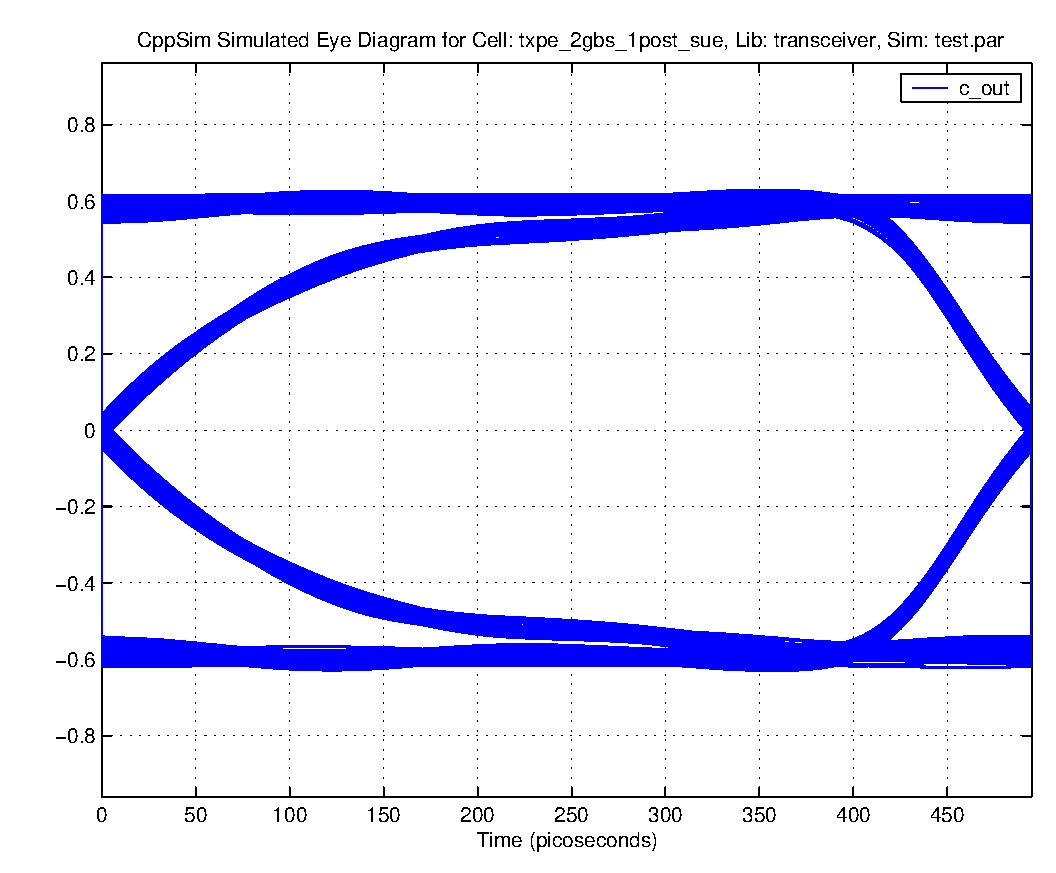
\includegraphics[scale=0.5]{eyes/eye_2gbs_1post.eps}}
  \subfigure[TXPE, two post cursors]
  {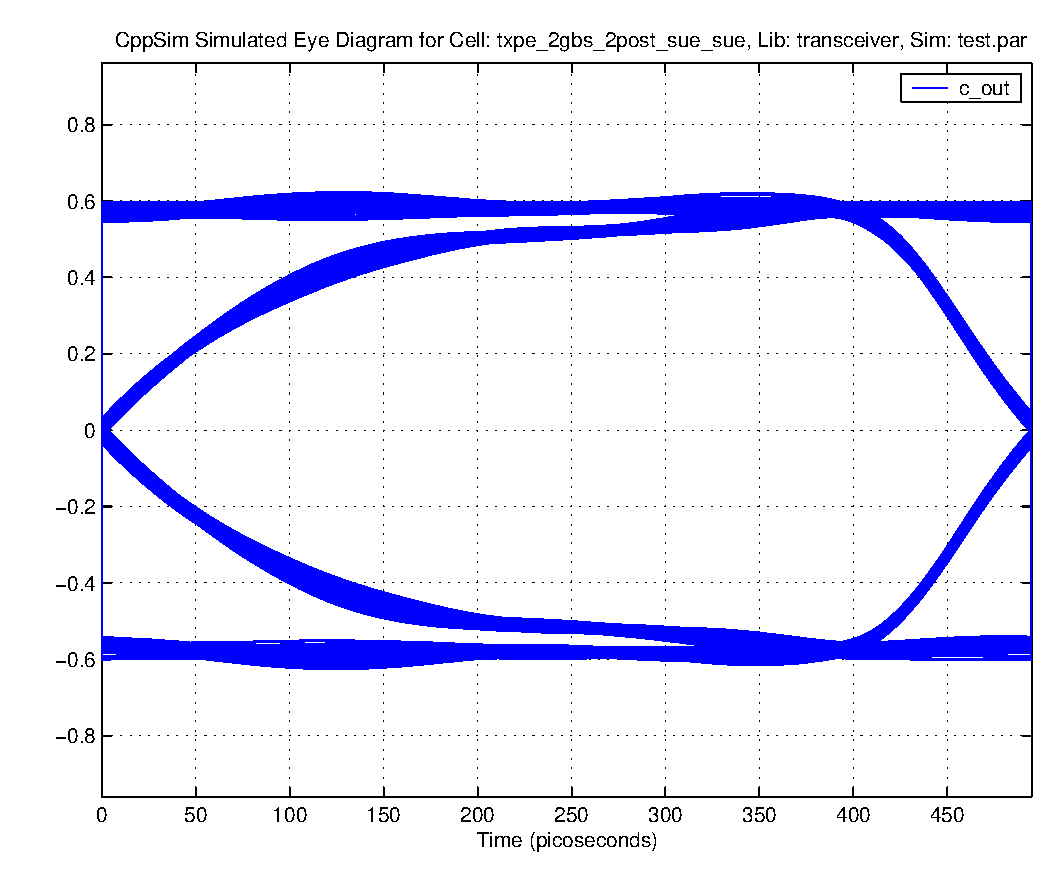
\includegraphics[scale=0.5]{eyes/eye_2gbs_2post.eps}}
  \caption{Eye diagrams for \unit[2]{Gb/s} and \unit[$\pm$0.7]{V} TX signal swing}
  \label{fig:eyes_2gbs}
\end{figure}
\subsection{Choice of clocking rate}
After investigation of several papers on high-speed links, we have decided to use a half-rate clocking scheme. Several sources ~\cite{rajesh2011a} ~\cite{palermo2010a} ~\cite{cressler2007a} cite half-rate clocking as being more power efficient in terms of clock-generation and distribution than a full-rate clock, some of these papers also point out that the power burned in the transmitter multiplexer can be a problem when dealing with quarter-rate clocking or lower. One of the largest motivators for choosing half-rate clocking in the preliminary design is due to the graph in figure \ref{fig:graph}. In this graph the distribution of clocking-schemes across different bit-rates and clock-frequencies can be observed, and it is clear that at 10Gb/s the half- and full-rate clocking schemes are the most used.

\begin{figure}[H]
\begin{center}
\includegraphics[scale=1.2]{img/clock0}
\caption{Use of different clock-rates in different implementations, source: ~\cite{rajesh2011a}}
\label{fig:graph}
\end{center}
\end{figure}

Taking a look at the graph in figure \ref{fig:graph1} the distribution of used clocking schemes in different technologies and their power consumption can be observed.

\begin{figure}[H]
\begin{center}
\includegraphics[scale=1.2]{img/clock1}
\caption{Distribution of different clock-rates in different technologies and their FOM, source: ~\cite{rajesh2011a}}
\label{fig:graph1}
\end{center}
\end{figure}

From the graph in figure \ref{fig:graph1} it can be observed that the half-rate clocking scheme is the most used in the 65nm process, and is also the clocking-rate that achieves the best power efficiency.

The half-rate clocking will be used at both the Tx and Rx side of the implementation in order to keep the design simple.

\subsection{Worst-case bit patterns}

The worst-case bit pattern for the channel running at 10Gb/s was generated by rendering the pulse response of the channel using the convolution of a 100ps pulse and the impulse response of the channel. A truncated plot of the resulting output is depicted in figure \ref{fig:worst}.


\begin{figure}[ht!]
\begin{center}
\includegraphics[scale=0.8]{img/graph}
\caption{Truncated pulse reponse of the channel, with the cursors marked as 'o's.}
\label{fig:worst}
\end{center}
\end{figure}

From the pulse response the worst-case bit pattern for transmitting a 
'1' was determined using the method learned in class, which is to flip the pulse response vertically and then using the highest peak as the cursor and each point an UI away as post/pre-cursors. If a post/pre-cursor has a positive value the corresponding bit in the pattern should be a '0', and a negative value yields a '1'.

The resulting worst-case bit pattern for a '1' around the cursor is shown in figure \ref{eq:wc}, where the cursor is the underlined '1'. The worst-case bit pattern for a '0' can be obtained by negating the bit-sequence for the worst-case '1'.


\begin{figure}[H]
$$\left[0,1,1,0,0,0,0,0,0,1,0,1,0,0,0,0,0,0,1,0,\underline{1},0,1,1,1,0,1,1,1,1,1,1,1,1,1,1,1,1,1,1,1,1\right]$$
\caption{Worst-case bit pattern for transmitting a '1' on the transmission line, the cursor is the underlined '1' in the pattern.}
\label{eq:wc}

\end{figure}



The used method yields the worst-case bit pattern with regard to eye-height, a worst-case bit pattern can also be determined to test the eye-width, this is described in ~\cite{designcon2011a}.

If worst-case bit-patterns for the other speeds of the transmission line are wanted, rendering it is a matter of using a different length pulse and use the UI for that pulse to determine the taps.

\cleardoublepage
\section{TX design}

\subsection{Choice of the circuit topology}

A specified for this assignment we need to design a:

\textit{Low-power supply-scalable (0.7-1.0V) I/O Link operating at 2-10Gb/s with at
least 2-tap voltage-mode TX. Minimize energy efficiency of the link, with an upper target
of 1pJ/b at 10Gb/s. }

So for the TX driver we first of all need to design a VM driver, for this we've chosen to use a slice topology in order to obtain a differential TX driver with equalization and tunable impedance.

For the TX driver we've decided to design for the topology depicted in figure \ref{fig:topology_tx}, where the serializer is responsible for serializing the input data to the transmitter, the two signals on each bus from the serializer to the TX driver is the cursor and the first post-cursor, the post-cursor is needed for serialization. The clock is a half-rate clock and thus it has two lines to the driver and serializer. The TX driver is as mentioned a slice design, where we've decided on using 12 slices in total, 9 for the cursor and 3 slices for the post-cursor. The reason we've decided to split up the allocation of slices is that this will lower the load for the pre-drivers.

\begin{figure}[H]
  \centering
  {\includegraphics[scale=0.55]{img/topology_tx.png}}
  \caption{Transmitter top level topology}
  \label{fig:topology_tx}
\end{figure}

The topology design is based on the half-rate transmitter design from ~\cite{menolfi2007a}, also depicted in figure \ref{fig:topology1}, we will however only feature one tap with a known sign, which will result in a simpler architecture.

\begin{figure}[H]
  \centering
  {\includegraphics[scale=0.55]{img/topology_tx1.png}}
  \caption{Transmitter top level topology from ~\cite{menolfi2007a}}
  \label{fig:topology1}
\end{figure}


The slice design we're going to use is based on the design used in ~\cite{menolfi2007a}, also depicted in figure \ref{fig:topology0}, as this is a slice designed for half-rate clocking operation hence very fitting to the design choices we made earlier.

\begin{figure}[H]
  \centering
  {\includegraphics[scale=0.55]{img/topology_tx0.png}}
  \caption{Half-rate slice topology from ~\cite{menolfi2007a}}
  \label{fig:topology0}
\end{figure}


\input{tx_schematics}
\subsection{Output signals for different input signals}

To prove that the transmitter works correctly and to obtain performance results the output for different input signals was observed. Figure \ref{fig:alternating_data} shows the transient waveform for alternating data at the TX output for \unit[6]{UI}. The eye diagram over \unit[5000]{UI} for a PRBS15 data pattern is given by figure \ref{fig:eye_prbs15}. The eye is not shown for \unit[10000]{UI} as we ran out of disk space and therefore could not run the simulation longer (we have to use cadence on the SOC machine where we only have a quota of \unit[4]{GB}).\\
In figure \ref{fig:wc_eye} the eye for the worst case data pattern of the transmitter is drawn. All bits transmitted in the simulation are shown in the eye diagram. As we used a long wc pattern this results in many traces. Only the two which close the eye the most are the actual worst-case one and zero bits of all bits transmitted for the worst-case pattern.

\begin{figure}[H]
  \centering
  \subfigure[with {\unit[6]{dB}} equalization]
  {\includegraphics[scale=0.3]{img/alternating_data.jpg}}
  \subfigure[equalization turned off]
  {\includegraphics[scale=0.3]{img/alternating_data_no_eq.jpg}}
  \caption{Transmitter output for alternating data at the input}
  \label{fig:alternating_data}
\end{figure}

\begin{figure}[H]
  \centering
  {\includegraphics[scale=0.4]{img/eye_rx_10gbs_5000.jpg}}
  \caption{Eye diagram over \unit[5000]{bits} for PRBS15 data pattern}
  \label{fig:eye_prbs15}
\end{figure}

\begin{figure}[H]
  \centering
  {\includegraphics[scale=0.35]{img/wc_eye_tx.jpg}}
  \caption{Worst case eye diagram at the transmitter output}
  \label{fig:wc_eye}
\end{figure}
\section{Impedance tuning}

To tune the output impedance of the transmitter the number of enabled slices can be varied. Reasonable values range from 4 to 12 slices. The resulting output impedance values for different numbers of enables slices are shown in figure \ref{fig:imp_tuning}. Please note that not with all these numbers of enabled slices the desired equalization can be reached exactly.

%TODO tuning range graph


\begin{figure}[H]
  \centering
  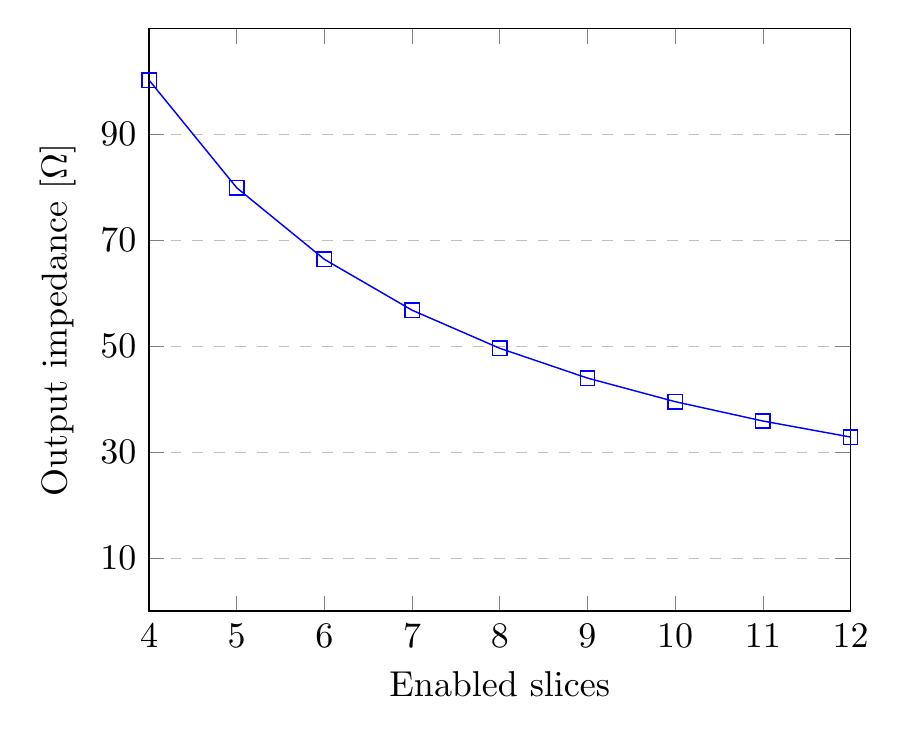
\begin{tikzpicture}[scale=1.3]
  \begin{axis}[
    %title={Output impedance tuning range},
    xlabel={Enabled slices},
    ylabel={Output impedance [$\Omega$]},
    xmin=4, xmax=12,
    ymin=0, ymax=110,
    xtick={4,5,6,7,8,9,10,11,12},
    ytick={10,30,50,70,90},
    ymajorgrids=true,
    grid style=dashed,
  ]

  \addplot[
    color=blue,
    mark=square,
    ]
    coordinates {
    (4,100.24)(5,79.92)(6,66.41)(7,56.81)(8,49.62)(9,44.00)(10,39.55)(11,35.90)(12,32.87)
    };

  \end{axis}
  \end{tikzpicture}
  \caption{Output impedance tuning range}
  \label{fig:imp_tuning}
\end{figure}


\subsection{Power consumption}

The power consumption at \unit[10]{Gb/s} PRBS15 data and \unit[1]{V} power supply as well as at \unit[2]{Gb/s} and \unit[0.7]{V} power supply is shown in table \ref{tab:power_consumption_tx}. The different power consumption between main and post cursors slices comes from the different input signal shapes as the post cursor is driven by the second flipflops whereas the main cursor slices are driven by the first flipflops for odd and even bits. The circuits of both slices are identical.

\begin{table}[H]
  \centering
  \begin{tabular}{l|r|r}
    component & \unit[10]{Gb/s} at \unit[1]{V} & \unit[2]{Gb/s} at \unit[0.7]{V}\\
    \hline
    complete transmitter &  \unit[37,933]{\uW} & \unit[5,720]{\uW}\\
    clock buffers & \unit[23,523]{\uW} &  \unit[2,221]{\uW}\\
    tap flipflops (used as pre-drivers) & \unit[3,610]{\uW} &  \unit[390]{\uW}\\
    main cursor slice &  \unit[1,239]{\uW} &  \unit[377]{\uW}\\
    main slice (inactive) &  \unit[1.548]{\uW} &  \unit[0.4]{\uW}\\
    post cursor slice &  \unit[1,189]{\uW} &  \unit[423]{\uW}\\
    post slice (inactive) &  \unit[1.802]{\uW} &  \unit[0.4]{\uW}\\      
  \end{tabular}
  \caption{Transmitter power consumption with PRBS15 data}
  \label{tab:power_consumption_tx}
\end{table}


\cleardoublepage
\section{RX design}

\section{Choice of the circuit topology}

\IEEEPARstart{A}{s} specified for this assignment we need to design a:

\textit{Low-power supply-scalable (0.7-1.0V) I/O Link operating at 2-10Gb/s with at
least 2-tap voltage-mode TX. Minimize energy efficiency of the link, with an upper target
of 1pJ/b at 10Gb/s. }

So for the TX driver we first of all need to design a VM driver, for this we've chosen to use a slice topology in order to obtain a differential TX driver with equalization and tunable impedance. To aid in the impedance tuning and lowering the power consumption we also seek to implement a shunt as well (this isn't included in the schematic in Cadence yet!), the shunt we seek to implement will be a tunable shunt, such that we can use fewer slices in the TX driver. Using less slices should help lowering the load for the pre-drivers and as such lower the total power consumption.

So for the TX driver we've decided to design for the topology depicted in figure \ref{fig:topology}, where the serializer is responsible for serializing the input data to the transmitter, the two signals on each bus from the serializer to the TX driver is the cursor and the first post-cursor, the post-cursor is needed for serialization. The clock is a half-rate clock and thus it has two lines to the driver and serializer. The TX driver is as mentioned a slice design, where we've decided on using 12 slices in total, 9 for the cursor and 3 slices for the post-cursor. The reason we've decided to split up the allocation of slices is that this will lower the load for the pre-drivers.

\begin{figure}[H]
  \centering
  {\includegraphics[scale=0.55]{img/Topology.png}}
  \caption{Transmitter top level topology}
  \label{fig:topology}
\end{figure}

The topology design is based on the half-rate transmitter design from ~\cite{menolfi2007a}, also depicted in \ref{fig:topology1}, we will however only feature one tap with a known sign, which will result in a simpler architecture.

\begin{figure}[H]
  \centering
  {\includegraphics[scale=0.55]{img/topology1.png}}
  \caption{Transmitter top level topology from ~\cite{menolfi2007a}}
  \label{fig:topology1}
\end{figure}


The slice design we're going to use is based on the design used in ~\cite{menolfi2007a}, also depicted in \ref{fig:topology0}, as this is a slice designed for half-rate clocking operation hence very fitting to the design choices we made earlier.

\begin{figure}[H]
  \centering
  {\includegraphics[scale=0.55]{img/topology0.png}}
  \caption{Half-rate slice topology from ~\cite{menolfi2007a}}
  \label{fig:topology0}
\end{figure}

For the serializer we haven't decided upon a final design, as we are uncertain about how the data will be presented to the transmitter, this will however be decided in future work.
\section{Transmitter schematics}

The top-level schematic of our transmitter circuit is shown in figure \ref{fig:top_level}. To make the circuit simpler to read, blocks are used for the different parts and the schematics of these blocks are shown separately. The input flipflops are implemented as in figure \ref{fig:flipflop}. Figure \ref{fig:slices} contains the schematics of our output slices. Note that each differential slice (part a of figure \ref{fig:slices}) contains two single-ended slices (part b of figure \ref{fig:slices}). All used gates were implemented on transistor level as well, the schematics for them are shown in figure \ref{fig:gates}.\\
All transistor were scaled the necessary driving capabilities with minimal area requirements and minimal loading to the previous stage, so we tried to use the minimal possible width. To do the scaling we first scaled all pre-driving circuits very large to ensure good input signals at the output slices. Our output slices have to reach an impedance of \unit[50]{$\Omega$} for impedance matching with the channel for the nominal number of slices turned on (eight). This is done by using the MOS resistance and the additional discrete series resistor to get better linearity. As consequence each of our slices have to have a impedance of \unit[400]{$\Omega$} of which \unit[300]{$\Omega$} are contributed by the passive resistor. To figure out the appropriate output transistor scaling we started with an educated guess for the width, measured the output resistance and then calculated the needed widths. To verify the value we simulated the output resistance again.\\
After that we minimized the scaling of the previous driver stage consisting of NAND and NOR gates for the generation of the driver signals so that the signals are still reasonable good but these drivers are also not generating too much load on the previous stage as they are present per slice, so 12 times in the worst case. Then we scaled down the transistors in the flipflops so that they can still drive the driving gates in the slices directly but do not have a too large capacitance loading to the input signal.\\
The final transistor scalings used are shown in table \ref{tab:scaling}.

\begin{table}[ht]
  \centering
  \begin{tabular}{l|l|l}
    type & nmos size & pmos size\\
    \hline
    output driver & \unit[8]{\um} & \unit[24]{\um}\\
    slice driver gates NAND & \unit[3]{\um} & \unit[3]{\um}\\
    slice driver gates NOR & \unit[1]{\um} & \unit[4]{\um}\\
    enable inverter & \unit[200]{nm} & \unit[400]{nm}\\
    flipflop & \unit[6]{\um} & \unit[12]{\um}\\
  \end{tabular}
  \caption{Used transistor sizes}
  \label{tab:scaling}
\end{table}
%TODO explain sizing!! and give the values!

\begin{figure}[ht]
  \centering
  {\includegraphics[scale=0.55]{img/transmitter.png}}
  \caption{Transmitter top level circuit}
  \label{fig:top_level}
\end{figure}

\begin{figure}[ht]
  \centering
  \subfigure[Differential slice]
  {\includegraphics[scale=0.6]{img/diff_slice.png}}
  \subfigure[Single-ended slice]
  {\includegraphics[scale=0.5]{img/se_slice.png}}
  \caption{Slice circuits}
  \label{fig:slices}
\end{figure}

\begin{figure}[ht]
  \centering
  {\includegraphics[scale=0.47]{img/flipflop.png}}
  \caption{D-Flipflop}
  \label{fig:flipflop}
\end{figure}

\begin{figure}[ht]
  \centering
  \subfigure[Inverter]
  {\includegraphics[scale=0.5]{img/inverter.png}}
  \subfigure[NAND gate]
  {\includegraphics[scale=0.5]{img/nand.png}}
  \subfigure[NOR gate]
  {\includegraphics[scale=0.5]{img/nor.png}}
  \caption{Simple gate circuits}
  \label{fig:gates}
\end{figure}
\section{Simulations}
\label{sec:simulations}
Figure \ref{fig:strongARM_out} shows the output of the stongARM latch for alternating data at the input for \unit[6]{UI}. For the simulation a data pattern of 11001100 was feed into the input of the receiver. As we have two slices with half-rate clocking this results in alternating data for one of the slices. To degenerate the signal and take the limited bandwith of the channel into account a RC circuit was used at the receiver input resulting in the \textit{in+} and \textit{in-} signals. The \textit{set} and \textit{reset} signals are the direct outputs of the strongARM circuit and the \textit{RS\_out} signal is one of the RS-FlipFlop outputs.

The frequency response of the variable offset amplifier (VOA) is shown in figure \ref{fig:voa_freq} and its ac noise response is drawn in figure \ref{fig:voa_noise}.

\begin{figure}[H]
  \centering
  {\includegraphics[scale=0.35]{img/voa_freq.jpg}}
  \caption{VOA frequency response}
  \label{fig:voa_freq}
\end{figure}

\begin{figure}[H]
  \centering
  {\includegraphics[scale=0.35]{img/voa_noise.jpg}}
  \caption{VOA ac noise response}
  \label{fig:voa_noise}
\end{figure}

\begin{figure}[H]
  \centering
  {\includegraphics[angle=90, scale=0.45]{img/output_alt_trans.jpg}}
  \caption{Transient waveform for alternating data at the output of the strongARM latch}
  \label{fig:strongARM_out}
\end{figure}
\section{Impedance and offset tuning}

To tune the input impedance of the receiver the input consists of a fixed portion and six resistors which can be switched on, doubled in size between each of them (see section \ref{sec:rx_schematics}). The resulting input impedance values for different codes are shown in figure \ref{fig:rx_imp_tuning_range}. The tuning ranges from \unit[70]{$\Omega$} to \unit[130]{$\Omega$}. Note that this tuning is not linear but as the best code has to be searched for the running link anyway, this leads only to small performance degradation as the tuning is more coarse for higher impedance values as for lower values.

\begin{figure}[H]
  \centering
  {\includegraphics[scale=0.9]{plots/rx_inp_imp.png}}
  \caption{Receiver input impedance tuning range}
  \label{fig:rx_imp_tuning_range}
\end{figure}

The variable offset voltage amplifier enables cancellation of offset voltages (e.g. due to mismatch in the differential pair of the strongARM latch). The achieved offset voltage over input code is shown in figure \ref{fig:voa_offset}. It ranges from \unit[-100]{mV} to \unit[100]{mV} and is pretty much linear.

\begin{figure}[H]
  \centering
  {\includegraphics[scale=0.9]{plots/voa_offset.png}}
  \caption{VOA offset voltage tuning range}
  \label{fig:voa_offset}
\end{figure}

\section{Power consumption}
The power consumption at \unit[10]{Gb/s} PRBS15 data and \unit[1]{V} power supply is shown in table \ref{tab:power_consumption}. The complete receiver consists of two receiver slices, each of them of VOA, strongARM and RS-FlipFlop (see section \ref{sec:rx_schematics}).

\begin{table}[H]
  \centering
  \begin{tabular}{l|l}
    component & consumed power\\
    \hline
    complete receiver & \unit[2104]{\uW}\\
    clock buffers & \unit[1814]{\uW}\\
    receiver slice & \unit[136,3]{\uW}\\
    VOA & \unit[32,58]{\uW}\\
    strongARM & \unit[46,07]{\uW}\\
    RS-FlipFlop & \unit[57,66]{\uW}\\
  \end{tabular}
  \caption{Receiver power consumption at \unit[10]{Gb/s} PRBS15 data and \unit[1]{V} power supply}
  \label{tab:power_consumption}
\end{table}
\section{Receiver specifications table }

In table \ref{tab:specifications} the specifications for the receiver is listed


\begin{table}[H]
  \centering
  \begin{tabular}{l|l|l|l|l}
    & Min. & Max. & Avg. & Unit \\
    \hline
	Termination impedance & 70 & 130 & 100 & $\Omega$\\
	Impedance resolution & 0.0087 & 2.289 & 0.858 & $\Omega$\\
	VOA offset & -100 & 100 & 0.0 & mV\\
	Offset resolution & 2.55 & 8.03 & 3.19 & mV\\
  \end{tabular}
  \caption{Partial specification table for the receiver}
  \label{tab:specifications}
\end{table}

The resolution of the Impedance and Offset both have a maximum and minimum value in the table, as some steps are smaller than others, due to the tuning not being perfectly linear, the max value do give an indication of the worst case scenario.

%TODO table with performance/specs


\cleardoublepage
\section{Link design and system tuning}
\subsection{Final link}



%TODO plots of the final link with 10,000UI and of WC-bit pattern, furthermore the BER of the link
\subsection{Link optimizations}
\label{sec:link_opt}
At first our link did not work. From simulations with equalization turned on and off and observing the eye diagram at the receiver input we could see that our equalization closed the eye instead of improving it. Debugging the schematics revealed that we implemented the tap with a positive sign instead of a negative sign and as result amplified the ISI of this cursor instead of canceling it. After changing the sign the equalization worked as expected.\\
After that we still got a lot of bit errors. As the input of the receiver was sufficient for the faulty bits we took a closer look at the intermediate signals in the receiver circuit. We figured out that the signal after our track-and-hold followed the input perfectly in the track phase. In the hold phase the differential signal was still maintained but the common mode of it made a significant step down towards the ground potential. Looking at the output of the following VOA in our design showed that this low common mode in the hold phase was to low for the amplifier to work and as consequence it only amplified the input signal in the track phase but not the hold phase, see figure \ref{fig:track_and_hold_problem} for the signals.

\begin{figure}[H]
  \centering
  {\includegraphics[scale=0.4]{img/track_and_hold_problem.png}}
  \caption{Track-and-hold common mode problem}
  \label{fig:track_and_hold_problem}
\end{figure}

This resulted in only half the time for the outputs to settle and would require double the bandwith for this amplifier than what we designed it for. This problem occured as we only used parasitic capacitances to implement the track-and-hold capacitance. The important capacitances here are the gate-source capacitance of the VOA input and the drain-bulk capacitance of the track-and-hold transistor. When the circuit now enters the hold phase the input is almost floating and only connected to these capacitances. As the source terminal of the VOA steers to ground now, the bulk is connected to $\overline{clk}$ and the voltage over the capacitors stays constant, the potential at the other terminal goes down. In other words, the reference potential changes.\\
To overcome this problem we added an extra capacitance of \unit[20]{fF} to the track-and-hold. This is approximatly five times larger than the parasitic capacitances and always connected to the same reference potential (GND), therefore the output stays almost constant between track and the hold phase.

\subsection{Performance results of final link}

The link simulated without any bit errors over \unit[5000]{UI} at \unit[2]{Gb/s} at \unit[1]{V}. For \unit[10]{Gb/s} at \unit[0.7]{V} we got 43 bit errors on the 5000 bits which clearly is a rather high BER, and not acceptable for a link like this. We assume that this is still the common mode problem of the track-and-hold described in section \ref{sec:link_opt} and that increasing the track-and.hold capacitor size would resolve these errors. However, due to our limited disk space quota we were not able to run more simulations on that and solve the problem.


The specifications of the link is listed in table \ref{tab:final_specifications}.


\begin{table}[H]
  \centering
  \begin{tabular}{l l|r|r|r|r}
 Unit  & Parameter & Min. & Max. & Avg. & Unit \\
    \hline
    & & & & &\\
\textbf{TX} & & & & &\\
&	Slice impedance & 400 &  &  & $\Omega$\\
&	No. of tap slices & 3 &  & 2 & \\
&	No. of cursor slices & 9 &  & 6 & \\
&	Output impedance range & 33.33 & 400 & 50 & $\Omega$\\
&	Power consumption at 2Gb/s 0.7V &  &  & 5,720 & $\mu$W\\
&	Power consumption at 10Gb/s 1.0V &  &  & 37,933 & $\mu$W\\

    & & & & &\\
   	\hline
    & & & & &\\
\textbf{RX} & & & & &\\
&	Termination impedance & 70 & 130 & 100 & $\Omega$\\
&	Impedance resolution & 0.0087 & 2.289 & 0.858 & $\Omega$\\
&	VOA offset & -100 & 100 & 0.0 & mV\\
&	Offset resolution & 2.55 & 8.03 & 3.19 & mV\\
&	Power consumption at 2Gb/s 0.7V &  &  & 223  & $\mu$W\\
&	Power consumption at 10Gb/s 1.0V &&  &  2,217  & $\mu$W\\

    & & & & &\\
    \hline
    & & & & &\\
\textbf{Link} & & & & &\\
&	Link speed & 2 & 10 &  & Gb/s \\
&	Supply voltage  & 0.7 & 1.0 &  & V\\
&	BER at 10Gb/s  &  &  & 0.0086 & \\
&	Power consumption at 2Gb/s 0.7V &  &  & 5,943 & $\mu$W\\
&	Power consumption at 10Gb/s 1.0V &  &  & 40,150 & $\mu$W\\
&   Energy per bit at 2Gb/s &  & & 2.9715 & pJ \\
&   Energy per bit at 10Gb/s &  & & 4.015 & pJ \\
  \end{tabular}
  \caption{Specification table of the link}
  \label{tab:final_specifications}
\end{table}


\section{Conclusion}
In this project we applied a lot of the material that we learned in the course over the time of the term. The result was a functional link implementation in Cadence Virtuoso where we obtained a link capable of running at different voltages in the range of 0.7-1.0V at different speeds in the range of 2-10Gb/s. The link had a BER of 0.0086 for a 5000UI simulation at 10Gb/s with a 1.0V power supply. The energy consumption of the link was however a factor of 4 above the desired goal of 1pJ/bit, looking at where the power was consumed it is clear that the transmitter of our link needs to be redesigned. It is evident that it is or clock distribution that consumes a lot of power, as well as the flip-flops that are used as pre-drivers for the TX driver, the problem probably lies in our choice of clock distribution as well as our scaling of the entire TX side of the link.


%\input{performance}



% Can use something like this to put references on a page
% by themselves when using endfloat and the captionsoff option.
\ifCLASSOPTIONcaptionsoff
  \newpage
\fi

\newpage
\section{Bibliography}
\bibliography{biblio}{}
\bibliographystyle{plain}


\end{document}


